\documentclass[a4paper, article, oneside, USenglish, IN5460]{memoir}

%% Title page
\usepackage{style/projectfp} 


%% Encoding
\usepackage[utf8]{inputenx} % Source code
\usepackage[T1]{fontenc}    % PDF


%% Fonts and typography
\usepackage{lmodern}           % Latin Modern Roman
\usepackage[scaled]{beramono}  % Bera Mono (Bitstream Vera Sans Mono)
\renewcommand{\sfdefault}{phv} % Helvetica
\usepackage[final]{microtype}  % Improved typography
\renewcommand{\abstractnamefont}{\sffamily\bfseries}                 % Abstract
\renewcommand*{\chaptitlefont}{\Large\bfseries\sffamily\raggedright} % Chapter
\setsecheadstyle{\large\bfseries\sffamily\raggedright}               % Section
\setsubsecheadstyle{\large\bfseries\sffamily\raggedright}            % Subsection
\setsubsubsecheadstyle{\normalsize\bfseries\sffamily\raggedright}    % Subsubsection
\setparaheadstyle{\normalsize\bfseries\sffamily\raggedright}         % Paragraph
\setsubparaheadstyle{\normalsize\bfseries\sffamily\raggedright}      % Subparagraph

%% Mathematics
\usepackage{amssymb}   % Extra symbols
\usepackage{amsthm}    % Theorem-like environments
\usepackage{thmtools}  % Theorem-like environments
\usepackage{mathtools} % Fonts and environments for mathematical formuale
\usepackage{mathrsfs}  % Script font with \mathscr{}

\title{Appliance Energy Consumption Prediction and Classification Using Federated Learning}
\authors{F. Ofstad, Z. Shan, R. Syed, H. Zhang}

\addbibresource{bibliography.bib}

\begin{document}

\projectfrontpage


\chapter{Introduction}
Appliance energy consumption is important for the stability of the smart grid system in a community. The prediction of energy consumption can help avoid the peak load. However, people in a community may not want to share their own data of energy consumption because of privacy protection. On the other hand, there may not be a server with enough capacity in the community. Therefore, Federated learning (FL) is a good approach for this scenario.

The purpose of this report is to construct a FL model, which aggregates the resulting weights from client models. The client models have two tasks:
\begin{enumerate}
    \item Train a model to predict the energy consumption for appliances in a household;
    \item Train a model to classify the type of appliance based on their energy consumption.    
\end{enumerate}

In both prediction and classification, we apply RNN and LSTM in implementing FL models. And then the performance of prediction and accuracy of classification of these two methods are analyzed respectively.

The dataset is an excel file includes $50$ sheets storing the energy consumption data of $50$ households. Each sheet records the $10$ appliance energy consumption for one year by period of every $15$ minutes. Besides, each household is regarded as a client that run one part of the distributed learning for FL model.


\chapter{Methodology}
To this end, we use Tensorflow package for Python when creating the client models using Keras, and the extension tensorflow federated for the aggregating model. The steps the program takes are as follows. 

\section{Pre-processing the data}
We first convert and segment the provided excel file into CSV files for each household. This is done to conceptually emulate FL as each client should only have access to their own data, and because CSV files are generally faster to load in Python.

Then for the prediction model, the data is processed as follows:
The applications energy consumption is summed up per period, creating a time-series dataset. This data set is segmented into pairs of seven days as inputs, with the $8$-th day being the output. In this way, we make data of every $8$ days as a sub-dataset. Then $20\%$ of the sub-datasets of each household are randomly selected for testing.

For the classification model, we focus on the energy consumption of appliance based on one day. As a result, every day's data ($96$ samples) is regarded as sub-dataset. So we can easily randomly choose $20\%$ of the days as test data.

\section{Training the models}

The clients themselves utilize RNN and LSTM models with n layers and n nodes #TODO-FILLIN
In prediction, we use $64$ nodes in both RNN and LSTM and only one hidden layer. 

The federated model runs these clients and extracts the averaged weights which it used for the aggregated model.



\chapter{Predicting Appliance Energy Consumption}

The following section tests the federated learning efficiency when predicting appliance energy consumption.

\section{Prediction with RNN}

\begin{figure}[H]
  \centering
    % This file was created with tikzplotlib v0.10.1.
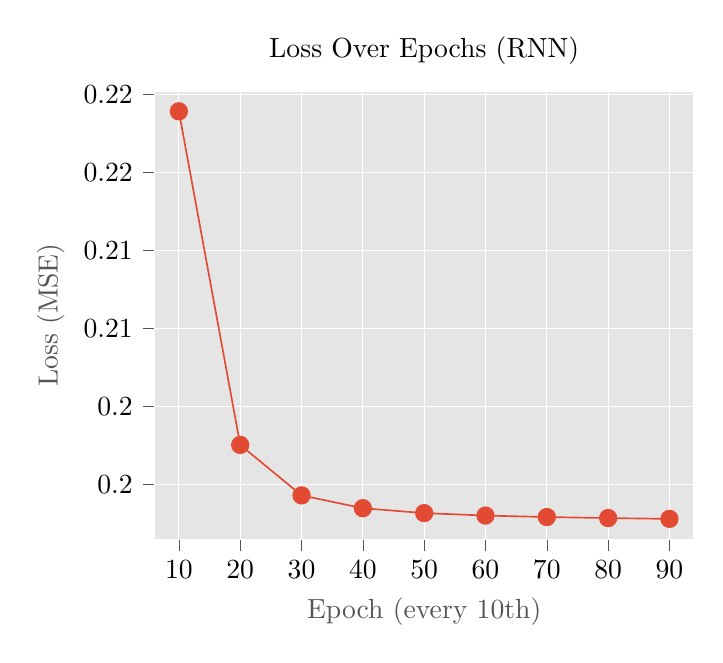
\begin{tikzpicture}

\definecolor{chocolate2267451}{RGB}{226,74,51}
\definecolor{dimgray85}{RGB}{85,85,85}
\definecolor{gainsboro229}{RGB}{229,229,229}

\begin{axis}[
axis background/.style={fill=gainsboro229},
axis line style={white},
tick align=outside,
tick pos=left,
title={Loss Over Epochs (RNN)},
x grid style={white},
xlabel=\textcolor{dimgray85}{Epoch (every 10th)},
xmajorgrids,
xmin=-0.4, xmax=8.4,
xtick style={color=dimgray85},
xtick={0,1,2,3,4,5,6,7,8},
xtick={0,1,2,3,4,5,6,7,8},
xticklabels={10,20,30,40,50,60,70,80,90},
xticklabels={10,20,30,40,50,60,70,80,90},
y grid style={white},
ylabel=\textcolor{dimgray85}{Loss (MSE)},
ymajorgrids,
ymin=0.191502721607685, ymax=0.220240204036236,
ytick style={color=dimgray85}
]
\addplot [semithick, chocolate2267451, mark=*, mark size=3, mark options={solid}]
table {%
0 0.218933954834938
1 0.197551742196083
2 0.194316670298576
3 0.193493545055389
4 0.193179294466972
5 0.193022191524506
6 0.192927539348602
7 0.19286160171032
8 0.192808970808983
};
\end{axis}

\end{tikzpicture}

  \caption{Simulation plot of the training error in MSE}
\end{figure}

As expected, the initial epochs provided the most reduction in loss, which starts to flatten out after around 40 epochs. After this there is minimal gain to be had by continuing the training. 

For the execution time, we found that adjusting the batch size contributed the most. Starting out with a small batch size extended the training time considerably, to the point where the run-time would timeout. But values in the 64 range, led to an execution time of 18min for 100 epochs.  

\begin{figure*}
        \centering
        \begin{subfigure}[b]{0.475\textwidth}
            \centering
            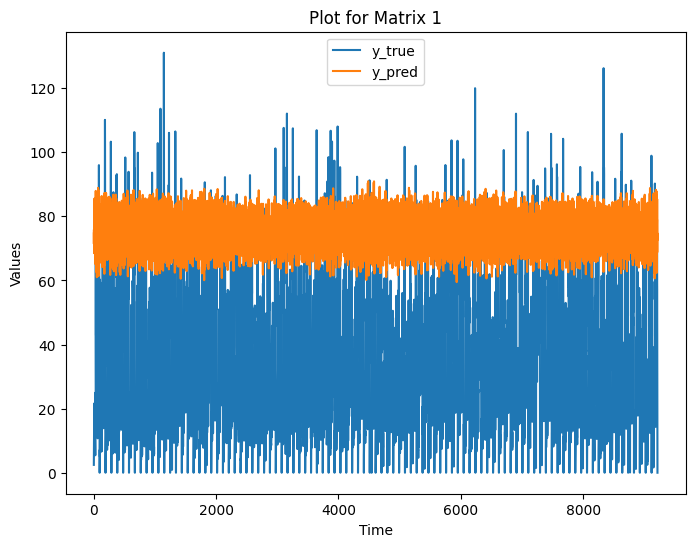
\includegraphics[width=\textwidth]{figures/RNN-pred/rnn1.png}
            {{\small Epoch 1}}    
        \end{subfigure}
        \hfill
        \begin{subfigure}[b]{0.475\textwidth}  
            \centering 
            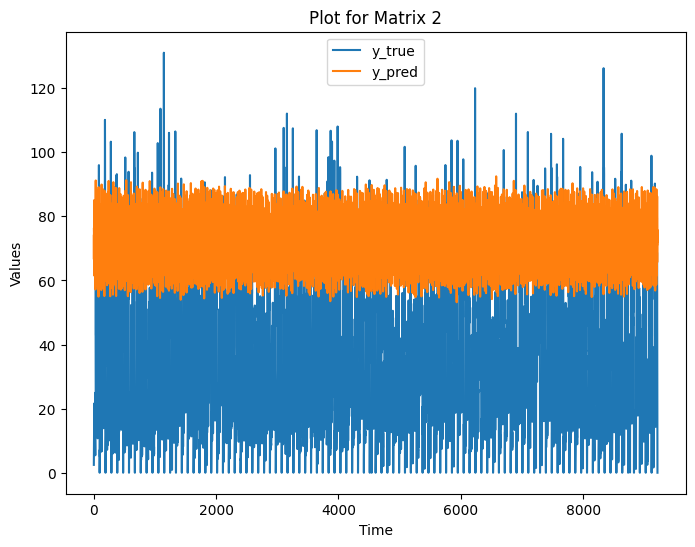
\includegraphics[width=\textwidth]{figures/RNN-pred/rnn2.png}
            {{\small Epoch 2}}    
        \end{subfigure}
        \vskip\baselineskip
        \begin{subfigure}[b]{0.475\textwidth}   
            \centering 
            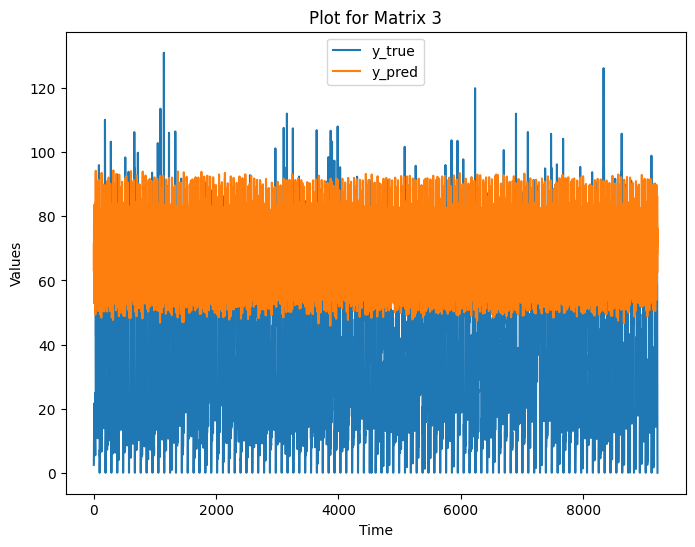
\includegraphics[width=\textwidth]{figures/RNN-pred/rnn3.png}
            {{\small Epoch 3}}    
        \end{subfigure}
        \hfill
        \begin{subfigure}[b]{0.475\textwidth}   
            \centering 
            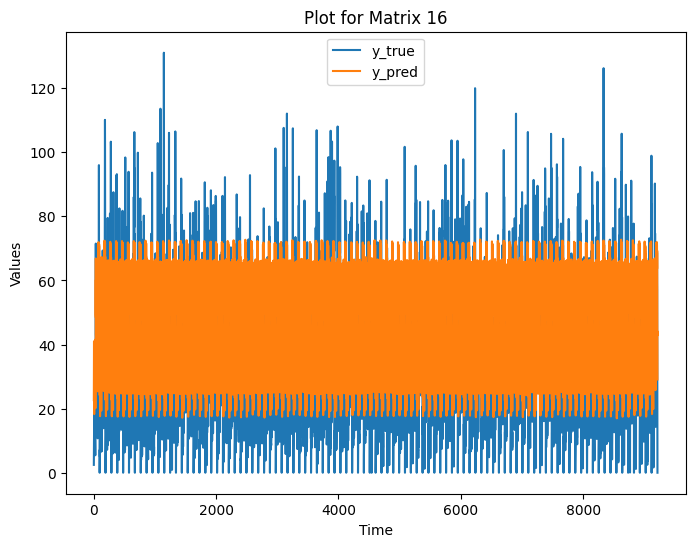
\includegraphics[width=\textwidth]{figures/RNN-pred/rnn16.png}
            {{\small Epoch 16}}
        \end{subfigure}
        \vskip\baselineskip
        \begin{subfigure}[b]{0.475\textwidth}   
            \centering 
            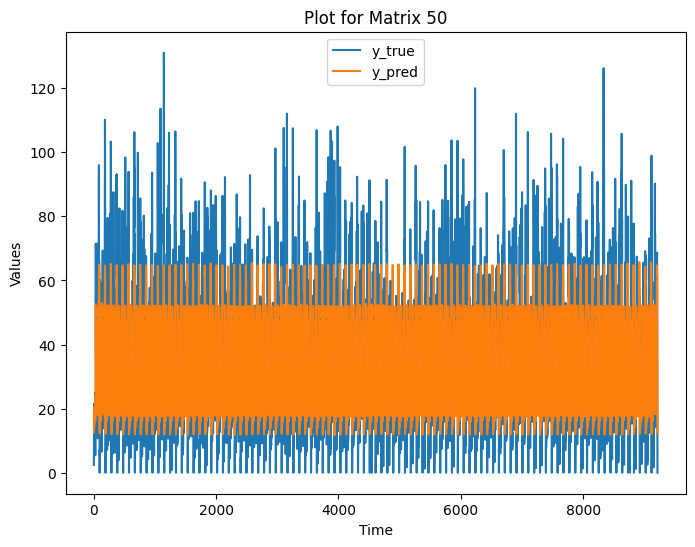
\includegraphics[width=\textwidth]{figures/RNN-pred/rnn50.png}
            {{\small Epoch 50}}    
        \end{subfigure}
        \hfill
        \begin{subfigure}[b]{0.475\textwidth}   
            \centering 
            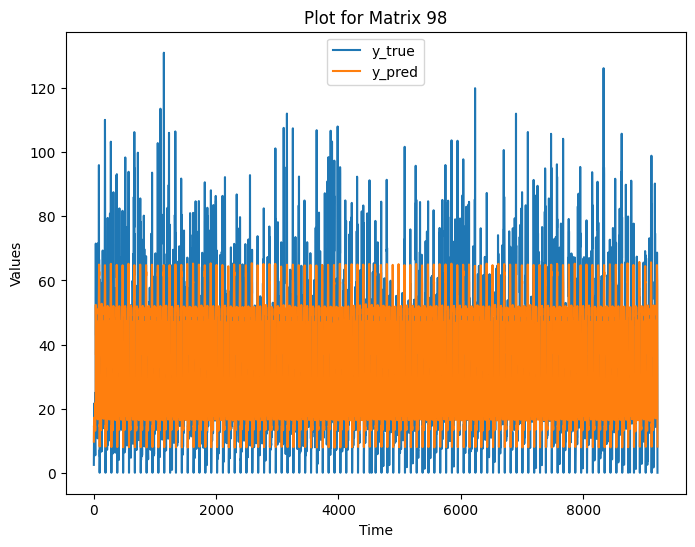
\includegraphics[width=\textwidth]{figures/RNN-pred/rnn98.png}
            {{\small Epoch 98}}
        \end{subfigure}
        \caption{RNN Prediction vs Ground Truth during different epochs in training} 
        \label{rnn-pred}
\end{figure*}

Figure \ref{rnn-pred} shows how the prediction of the energy value changes throughout the training epochs. Similar to the results shown in figure 1, the biggest gains are seen in the first couple of epochs. We can see that there isn't much difference in the prediction produced by the model in epoch 50 and 98. While some patterns are captured, The model seems to under-predict the energy.


\begin{figure}[H]
  \centering
    % This file was created with tikzplotlib v0.10.1.
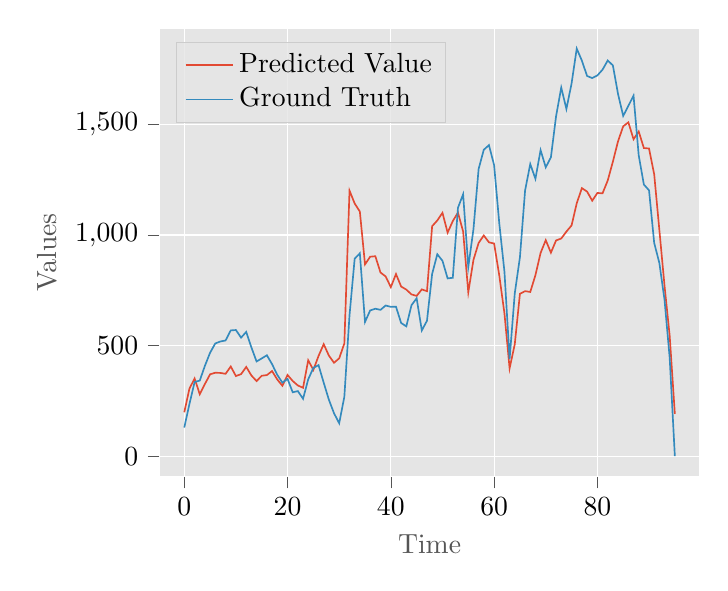
\begin{tikzpicture}

\definecolor{chocolate2267451}{RGB}{226,74,51}
\definecolor{dimgray85}{RGB}{85,85,85}
\definecolor{gainsboro229}{RGB}{229,229,229}
\definecolor{lightgray204}{RGB}{204,204,204}
\definecolor{steelblue52138189}{RGB}{52,138,189}

\begin{axis}[
axis background/.style={fill=gainsboro229},
axis line style={white},
legend cell align={left},
legend style={
  fill opacity=0.8,
  draw opacity=1,
  text opacity=1,
  at={(0.03,0.97)},
  anchor=north west,
  draw=lightgray204,
  fill=gainsboro229
},
tick align=outside,
tick pos=left,
x grid style={white},
xlabel=\textcolor{dimgray85}{Time},
xmajorgrids,
xmin=-4.75, xmax=99.75,
xtick style={color=dimgray85},
y grid style={white},
ylabel=\textcolor{dimgray85}{Values},
ymajorgrids,
ymin=-92.1626037597656, ymax=1935.41467895508,
ytick style={color=dimgray85}
]
\addplot [semithick, chocolate2267451]
table {%
0 198.435546875
1 305.348388671875
2 351.123596191406
3 280.257446289062
4 326.569091796875
5 370.180358886719
6 377.343719482422
7 376.40087890625
8 372.475738525391
9 405.539276123047
10 362.38134765625
11 370.920806884766
12 403.540588378906
13 364.933563232422
14 339.542297363281
15 363.637847900391
16 366.665252685547
17 384.902740478516
18 347.018432617188
19 318.433563232422
20 367.244812011719
21 339.870422363281
22 319.708190917969
23 309.245758056641
24 433.651580810547
25 390.149536132812
26 453.100219726562
27 506.504852294922
28 455.062927246094
29 422.359680175781
30 442.376708984375
31 509.964904785156
32 1200.81359863281
33 1142.65612792969
34 1106.35314941406
35 867.460571289062
36 901.951354980469
37 904.322814941406
38 830.587341308594
39 812.804077148438
40 764.389526367188
41 823.682739257812
42 767.180480957031
43 753.252502441406
44 731.552551269531
45 724.874206542969
46 754.290283203125
47 746.048278808594
48 1039.99963378906
49 1065.94799804688
50 1100.6025390625
51 1010.90161132812
52 1063.18933105469
53 1101.48229980469
54 1016.02459716797
55 741.026794433594
56 887.600708007812
57 964.327209472656
58 998.208618164062
59 967.022583007812
60 961.778259277344
61 817.461853027344
62 646.188659667969
63 396.981781005859
64 506.180969238281
65 734.420166015625
66 746.390686035156
67 742.519287109375
68 818.391174316406
69 919.016845703125
70 976.813232421875
71 920.355163574219
72 975.723083496094
73 984.385009765625
74 1015.71130371094
75 1043.39562988281
76 1143.63439941406
77 1212.20825195312
78 1196.73364257812
79 1155.51171875
80 1190.37890625
81 1188.79064941406
82 1246.54296875
83 1331.8662109375
84 1424.27600097656
85 1491.96276855469
86 1509.69458007812
87 1433.40051269531
88 1468.5234375
89 1393.54357910156
90 1391.48327636719
91 1275.0537109375
92 1023.29461669922
93 771.010620117188
94 544.187072753906
95 190.823638916016
};
\addlegendentry{Predicted Value}
\addplot [semithick, steelblue52138189]
table {%
0 129.466995239258
1 235.788040161133
2 335.239013671875
3 341.838958740234
4 408.933044433594
5 467.786010742188
6 509.720977783203
7 518.746948242188
8 523.286071777344
9 568.80615234375
10 570.518981933594
11 536.034057617188
12 561.9580078125
13 491.852081298828
14 428.232971191406
15 442.130004882812
16 456.27001953125
17 416.250061035156
18 367.885131835938
19 332.779968261719
20 349.243988037109
21 288.894012451172
22 294.340087890625
23 259.463012695312
24 347.286865234375
25 399.473541259766
26 411.618865966797
27 332.483306884766
28 255.468490600586
29 194.055541992188
30 148.838653564453
31 268.954803466797
32 637.510559082031
33 893.097900390625
34 917.37158203125
35 607.062194824219
36 659.185546875
37 666.920349121094
38 661.749267578125
39 681.366821289062
40 675.322570800781
41 675.73974609375
42 602.161743164062
43 586.995361328125
44 682.61181640625
45 713.9521484375
46 568.656127929688
47 612.405639648438
48 824.173767089844
49 913.189392089844
50 883.589294433594
51 803.853576660156
52 806.86767578125
53 1123.28039550781
54 1184.56921386719
55 855.762390136719
56 1026.18713378906
57 1298.71496582031
58 1385.69470214844
59 1406.73718261719
60 1316.287109375
61 1053.48266601562
62 835.051330566406
63 439.343688964844
64 735.6787109375
65 899.506713867188
66 1201.94165039062
67 1321.05944824219
68 1254.30261230469
69 1383.99926757812
70 1306.33471679688
71 1351.57092285156
72 1537.50439453125
73 1666.82348632812
74 1570.27392578125
75 1685.42407226562
76 1843.25207519531
77 1788.52404785156
78 1719.50329589844
79 1709.91394042969
80 1721.95104980469
81 1748.08654785156
82 1789.38952636719
83 1767.27990722656
84 1637.69860839844
85 1538.72326660156
86 1584.41137695312
87 1630.5771484375
88 1360.75805664062
89 1228.44470214844
90 1202.36315917969
91 964.465759277344
92 873.629699707031
93 707.248962402344
94 444.571258544922
95 0
};
\addlegendentry{Ground Truth}
\end{axis}

\end{tikzpicture}

  \caption{Simulation plot comparing the predicted value with the ground truth}
\end{figure}


%Is the federated learning efficient in this scenario of appliance energy consumption prediction? Please discuss whether the performance of model training can be improved by adding more epochs or through other configuration changes.


\section{Prediction with LSTM}

The following models use the same configurations as the previous model, except the trainer uses LSTM instead of regular RNN.

\begin{figure}[H]
  \centering
    % This file was created with tikzplotlib v0.10.1.
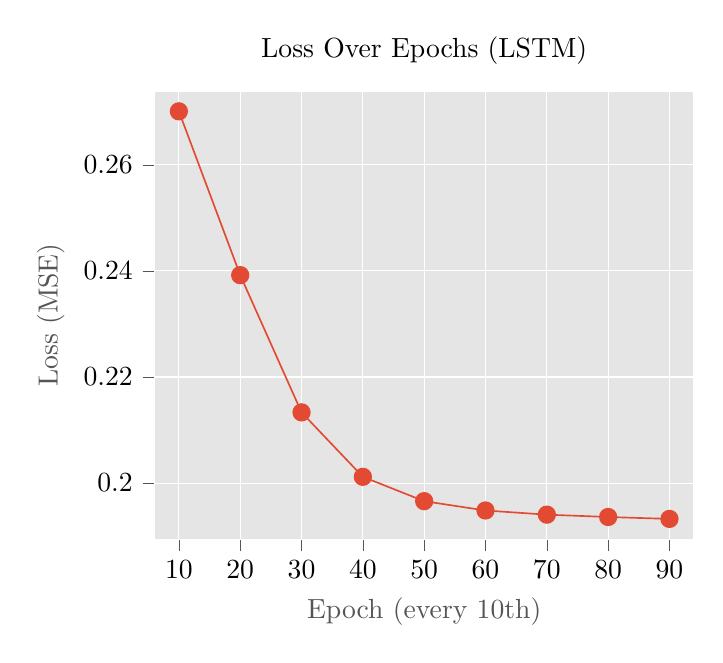
\begin{tikzpicture}

\definecolor{chocolate2267451}{RGB}{226,74,51}
\definecolor{dimgray85}{RGB}{85,85,85}
\definecolor{gainsboro229}{RGB}{229,229,229}

\begin{axis}[
axis background/.style={fill=gainsboro229},
axis line style={white},
tick align=outside,
tick pos=left,
title={Loss Over Epochs (LSTM)},
x grid style={white},
xlabel=\textcolor{dimgray85}{Epoch (every 10th)},
xmajorgrids,
xmin=-0.4, xmax=8.4,
xtick style={color=dimgray85},
xtick={0,1,2,3,4,5,6,7,8},
xtick={0,1,2,3,4,5,6,7,8},
xticklabels={10,20,30,40,50,60,70,80,90},
xticklabels={10,20,30,40,50,60,70,80,90},
y grid style={white},
ylabel=\textcolor{dimgray85}{Loss (MSE)},
ymajorgrids,
ymin=0.189402960240841, ymax=0.273933596909046,
ytick style={color=dimgray85}
]
\addplot [semithick, chocolate2267451, mark=*, mark size=3, mark options={solid}]
table {%
0 0.27009129524231
1 0.239204823970795
2 0.21332985162735
3 0.201177880167961
4 0.196588724851608
5 0.194829702377319
6 0.194046154618263
7 0.193602621555328
8 0.193245261907578
};
\end{axis}

\end{tikzpicture}

  \caption{Simulation plot of the training error in MSE}
\end{figure}

The LSTM model starts with a higher initial loss, and takes more epochs than the RNN model before the loss gradient flattens out.


\begin{figure*}
        \centering
        \begin{subfigure}[b]{0.475\textwidth}
            \centering
            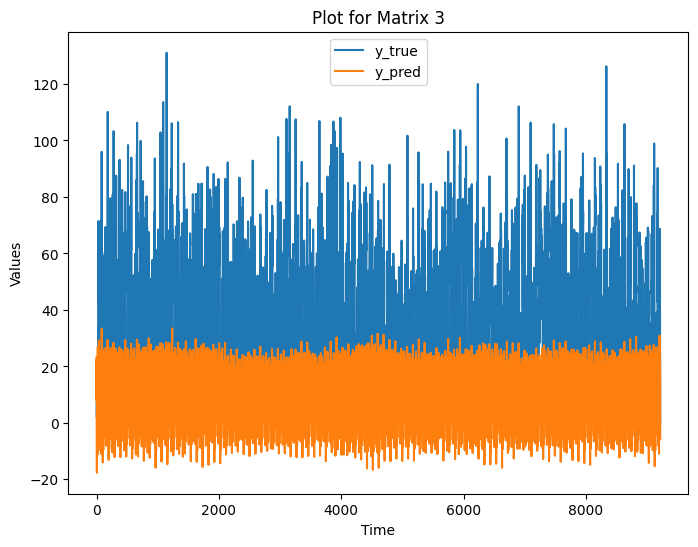
\includegraphics[width=\textwidth]{figures/LSTM-Pred/plot3.png}
            {{\small Epoch 3}}    
        \end{subfigure}
        \hfill
        \begin{subfigure}[b]{0.475\textwidth}  
            \centering 
            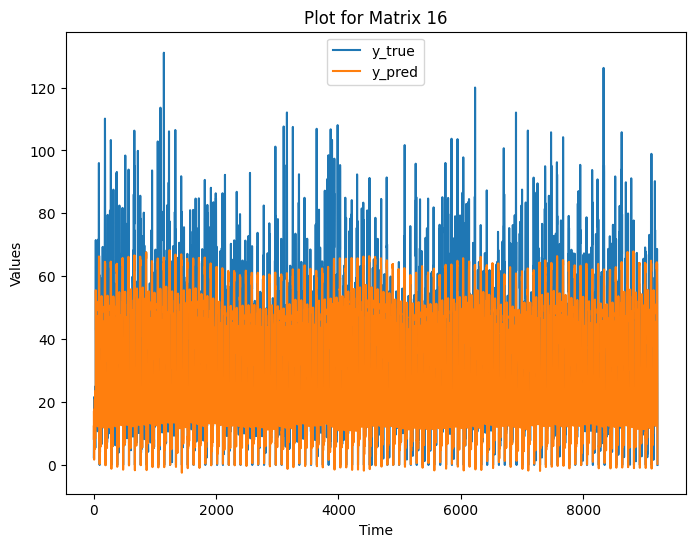
\includegraphics[width=\textwidth]{figures/LSTM-Pred/plot16.png}
            {{\small Epoch 16}}    
        \end{subfigure}
        \vskip\baselineskip
        \begin{subfigure}[b]{0.475\textwidth}   
            \centering 
            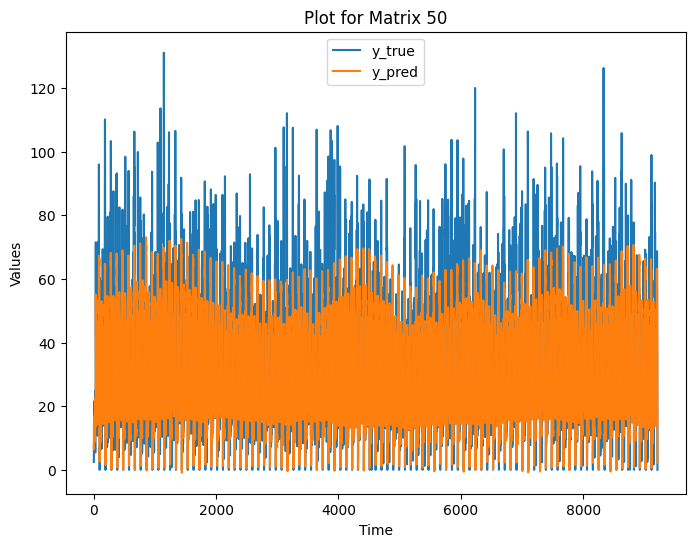
\includegraphics[width=\textwidth]{figures/LSTM-Pred/plot50.png}
            {{\small Epoch 50}}    
        \end{subfigure}
        \hfill
        \begin{subfigure}[b]{0.475\textwidth}   
            \centering 
            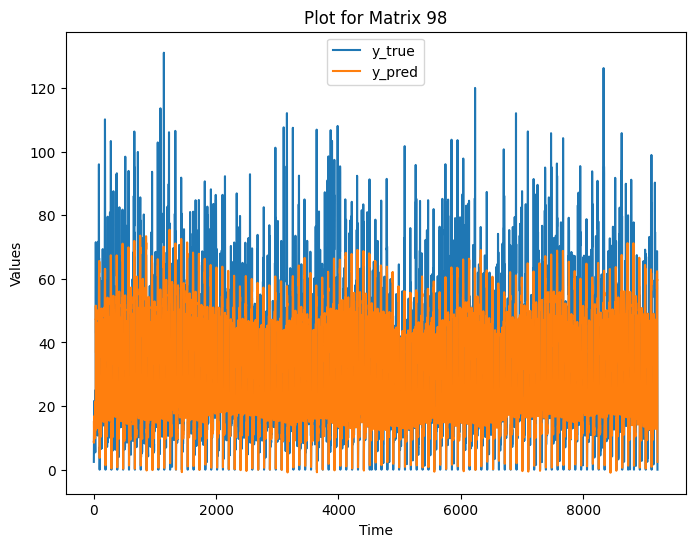
\includegraphics[width=\textwidth]{figures/LSTM-Pred/plot98.png}
            {{\small Epoch 98}}    
        \end{subfigure}
        \caption{LSTM Prediction vs Ground Truth during different epochs in training} 
        \label{lstm-pred}
\end{figure*}

Figure \ref{lstm-pred} shows that by epoch 16, the LSTM model already produces better predictions than the all the RNN models.

\begin{figure}[H]
  \centering
    % This file was created with tikzplotlib v0.10.1.
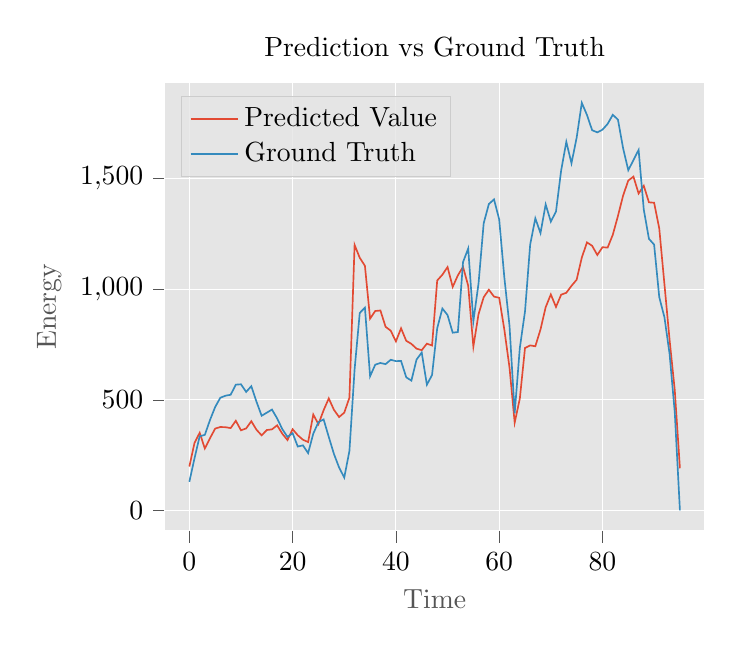
\begin{tikzpicture}

\definecolor{chocolate2267451}{RGB}{226,74,51}
\definecolor{dimgray85}{RGB}{85,85,85}
\definecolor{gainsboro229}{RGB}{229,229,229}
\definecolor{lightgray204}{RGB}{204,204,204}
\definecolor{steelblue52138189}{RGB}{52,138,189}

\begin{axis}[
axis background/.style={fill=gainsboro229},
axis line style={white},
legend cell align={left},
legend style={
  fill opacity=0.8,
  draw opacity=1,
  text opacity=1,
  at={(0.03,0.97)},
  anchor=north west,
  draw=lightgray204,
  fill=gainsboro229
},
tick align=outside,
tick pos=left,
title={Prediction vs Ground Truth},
x grid style={white},
xlabel=\textcolor{dimgray85}{Time},
xmajorgrids,
xmin=-4.75, xmax=99.75,
xtick style={color=dimgray85},
y grid style={white},
ylabel=\textcolor{dimgray85}{Energy},
ymajorgrids,
ymin=-92.1626037597656, ymax=1935.41467895508,
ytick style={color=dimgray85}
]
\addplot [semithick, chocolate2267451]
table {%
0 198.435546875
1 305.348388671875
2 351.123596191406
3 280.257446289062
4 326.569091796875
5 370.180358886719
6 377.343719482422
7 376.40087890625
8 372.475738525391
9 405.539276123047
10 362.38134765625
11 370.920806884766
12 403.540588378906
13 364.933563232422
14 339.542297363281
15 363.637847900391
16 366.665252685547
17 384.902740478516
18 347.018432617188
19 318.433563232422
20 367.244812011719
21 339.870422363281
22 319.708190917969
23 309.245758056641
24 433.651580810547
25 390.149536132812
26 453.100219726562
27 506.504852294922
28 455.062927246094
29 422.359680175781
30 442.376708984375
31 509.964904785156
32 1200.81359863281
33 1142.65612792969
34 1106.35314941406
35 867.460571289062
36 901.951354980469
37 904.322814941406
38 830.587341308594
39 812.804077148438
40 764.389526367188
41 823.682739257812
42 767.180480957031
43 753.252502441406
44 731.552551269531
45 724.874206542969
46 754.290283203125
47 746.048278808594
48 1039.99963378906
49 1065.94799804688
50 1100.6025390625
51 1010.90161132812
52 1063.18933105469
53 1101.48229980469
54 1016.02459716797
55 741.026794433594
56 887.600708007812
57 964.327209472656
58 998.208618164062
59 967.022583007812
60 961.778259277344
61 817.461853027344
62 646.188659667969
63 396.981781005859
64 506.180969238281
65 734.420166015625
66 746.390686035156
67 742.519287109375
68 818.391174316406
69 919.016845703125
70 976.813232421875
71 920.355163574219
72 975.723083496094
73 984.385009765625
74 1015.71130371094
75 1043.39562988281
76 1143.63439941406
77 1212.20825195312
78 1196.73364257812
79 1155.51171875
80 1190.37890625
81 1188.79064941406
82 1246.54296875
83 1331.8662109375
84 1424.27600097656
85 1491.96276855469
86 1509.69458007812
87 1433.40051269531
88 1468.5234375
89 1393.54357910156
90 1391.48327636719
91 1275.0537109375
92 1023.29461669922
93 771.010620117188
94 544.187072753906
95 190.823638916016
};
\addlegendentry{Predicted Value}
\addplot [semithick, steelblue52138189]
table {%
0 129.466995239258
1 235.788040161133
2 335.239013671875
3 341.838958740234
4 408.933044433594
5 467.786010742188
6 509.720977783203
7 518.746948242188
8 523.286071777344
9 568.80615234375
10 570.518981933594
11 536.034057617188
12 561.9580078125
13 491.852081298828
14 428.232971191406
15 442.130004882812
16 456.27001953125
17 416.250061035156
18 367.885131835938
19 332.779968261719
20 349.243988037109
21 288.894012451172
22 294.340087890625
23 259.463012695312
24 347.286865234375
25 399.473541259766
26 411.618865966797
27 332.483306884766
28 255.468490600586
29 194.055541992188
30 148.838653564453
31 268.954803466797
32 637.510559082031
33 893.097900390625
34 917.37158203125
35 607.062194824219
36 659.185546875
37 666.920349121094
38 661.749267578125
39 681.366821289062
40 675.322570800781
41 675.73974609375
42 602.161743164062
43 586.995361328125
44 682.61181640625
45 713.9521484375
46 568.656127929688
47 612.405639648438
48 824.173767089844
49 913.189392089844
50 883.589294433594
51 803.853576660156
52 806.86767578125
53 1123.28039550781
54 1184.56921386719
55 855.762390136719
56 1026.18713378906
57 1298.71496582031
58 1385.69470214844
59 1406.73718261719
60 1316.287109375
61 1053.48266601562
62 835.051330566406
63 439.343688964844
64 735.6787109375
65 899.506713867188
66 1201.94165039062
67 1321.05944824219
68 1254.30261230469
69 1383.99926757812
70 1306.33471679688
71 1351.57092285156
72 1537.50439453125
73 1666.82348632812
74 1570.27392578125
75 1685.42407226562
76 1843.25207519531
77 1788.52404785156
78 1719.50329589844
79 1709.91394042969
80 1721.95104980469
81 1748.08654785156
82 1789.38952636719
83 1767.27990722656
84 1637.69860839844
85 1538.72326660156
86 1584.41137695312
87 1630.5771484375
88 1360.75805664062
89 1228.44470214844
90 1202.36315917969
91 964.465759277344
92 873.629699707031
93 707.248962402344
94 444.571258544922
95 0
};
\addlegendentry{Ground Truth}
\end{axis}

\end{tikzpicture}

  \caption{Simulation plot comparing the predicted value with the ground truth}
\end{figure}

 %Compare the performance with that of RNN regarding execution time and prediction error during the test.

\chapter{Classifying Appliance Types}

This section reports the results of the classification model: determining the types of application based on the daily consumption of an appliance.

\section{Classification using Regular RNN}

\begin{figure}[H]
  \centering
    % This file was created with tikzplotlib v0.10.1.
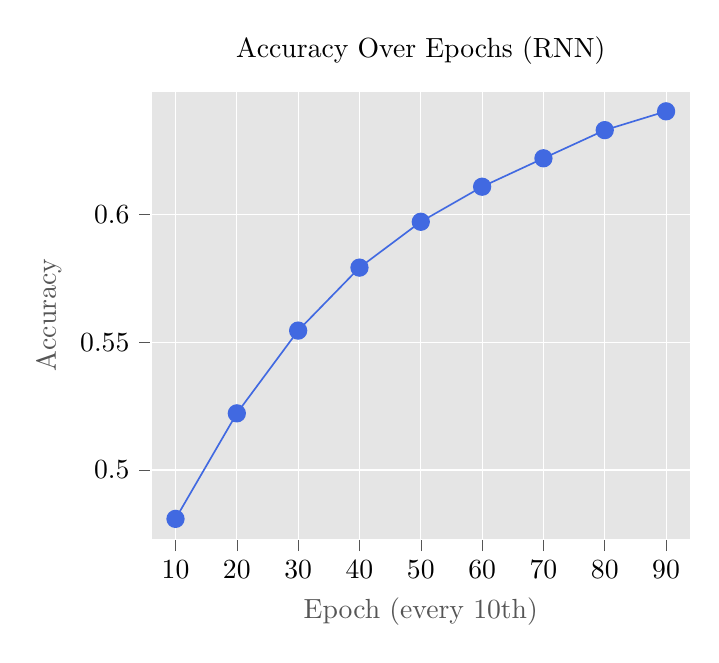
\begin{tikzpicture}

\definecolor{dimgray85}{RGB}{85,85,85}
\definecolor{gainsboro229}{RGB}{229,229,229}
\definecolor{royalblue}{RGB}{65,105,225}

\begin{axis}[
axis background/.style={fill=gainsboro229},
axis line style={white},
tick align=outside,
tick pos=left,
title={Accuracy Over Epochs (RNN)},
x grid style={white},
xlabel=\textcolor{dimgray85}{Epoch (every 10th)},
xmajorgrids,
xmin=-0.4, xmax=8.4,
xtick style={color=dimgray85},
xtick={0,1,2,3,4,5,6,7,8},
xtick={0,1,2,3,4,5,6,7,8},
xticklabels={10,20,30,40,50,60,70,80,90},
xticklabels={10,20,30,40,50,60,70,80,90},
y grid style={white},
ylabel=\textcolor{dimgray85}{Accuracy},
ymajorgrids,
ymin=0.472926071286201, ymax=0.648256549239159,
ytick style={color=dimgray85}
]
\addplot [semithick, royalblue, mark=*, mark size=3, mark options={solid}]
table {%
0 0.480895638465881
1 0.522173941135406
2 0.554530441761017
3 0.57916522026062
4 0.597095668315887
5 0.61080002784729
6 0.621921718120575
7 0.63293045759201
8 0.640286982059479
};
\end{axis}

\end{tikzpicture}

  \caption{Plot showing the change in accuracy during training}
\end{figure}

%Is the federated learning efficient in this scenario of appliance classification? Please use simulation plots to show the classification accuracy during the training process using training (or training and validation) data, and show the classification accuracy of the trained model using test data. Please discuss whether the accuracy during the training and testing can be improved by adding more epochs or through other configuration changes.

\section{Confusion Matrix}

\begin{figure}[H]
  \centering
    % This file was created with tikzplotlib v0.10.1.
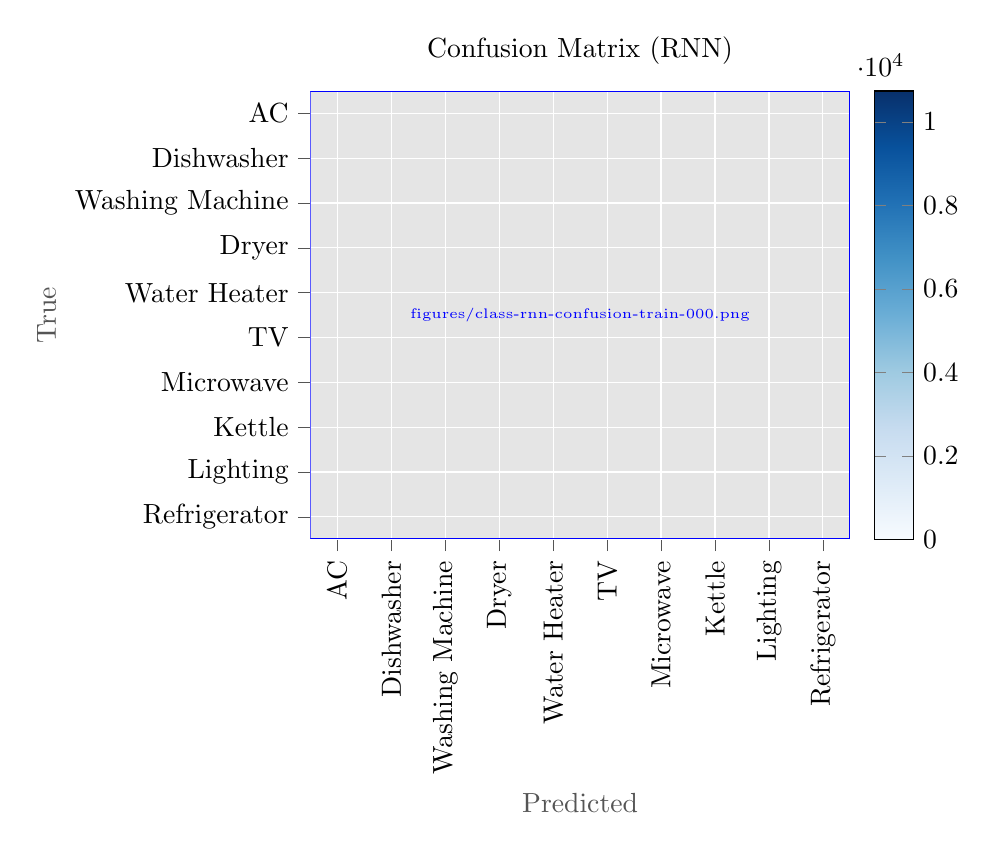
\begin{tikzpicture}

\definecolor{dimgray85}{RGB}{85,85,85}
\definecolor{gainsboro229}{RGB}{229,229,229}

\begin{axis}[
axis background/.style={fill=gainsboro229},
axis line style={white},
colorbar,
colorbar style={ylabel={}},
colormap={mymap}{[1pt]
  rgb(0pt)=(0.968627450980392,0.984313725490196,1);
  rgb(1pt)=(0.870588235294118,0.92156862745098,0.968627450980392);
  rgb(2pt)=(0.776470588235294,0.858823529411765,0.937254901960784);
  rgb(3pt)=(0.619607843137255,0.792156862745098,0.882352941176471);
  rgb(4pt)=(0.419607843137255,0.682352941176471,0.83921568627451);
  rgb(5pt)=(0.258823529411765,0.572549019607843,0.776470588235294);
  rgb(6pt)=(0.129411764705882,0.443137254901961,0.709803921568627);
  rgb(7pt)=(0.0313725490196078,0.317647058823529,0.611764705882353);
  rgb(8pt)=(0.0313725490196078,0.188235294117647,0.419607843137255)
},
point meta max=10741,
point meta min=0,
tick align=outside,
tick pos=left,
title={Confusion Matrix (RNN)},
x grid style={white},
xlabel=\textcolor{dimgray85}{Predicted},
xmajorgrids,
xmin=0, xmax=10,
xtick style={color=dimgray85},
xtick={0.5,1.5,2.5,3.5,4.5,5.5,6.5,7.5,8.5,9.5},
xticklabel style={rotate=90.0},
xticklabels={
  AC,
  Dishwasher,
  Washing Machine,
  Dryer,
  Water Heater,
  TV,
  Microwave,
  Kettle,
  Lighting,
  Refrigerator
},
y dir=reverse,
y grid style={white},
ylabel=\textcolor{dimgray85}{True},
ymajorgrids,
ymin=0, ymax=10,
ytick style={color=dimgray85},
ytick={0.5,1.5,2.5,3.5,4.5,5.5,6.5,7.5,8.5,9.5},
yticklabels={
  AC,
  Dishwasher,
  Washing Machine,
  Dryer,
  Water Heater,
  TV,
  Microwave,
  Kettle,
  Lighting,
  Refrigerator
}
]
\addplot graphics [includegraphics cmd=\pgfimage,xmin=0, xmax=10, ymin=10, ymax=0] {figures/class-rnn-confusion-train-000.png};
\end{axis}

\end{tikzpicture}

  \caption{Confusion Matrix for the training data}
\end{figure}

\begin{figure}[H]
  \centering
    % This file was created with tikzplotlib v0.10.1.
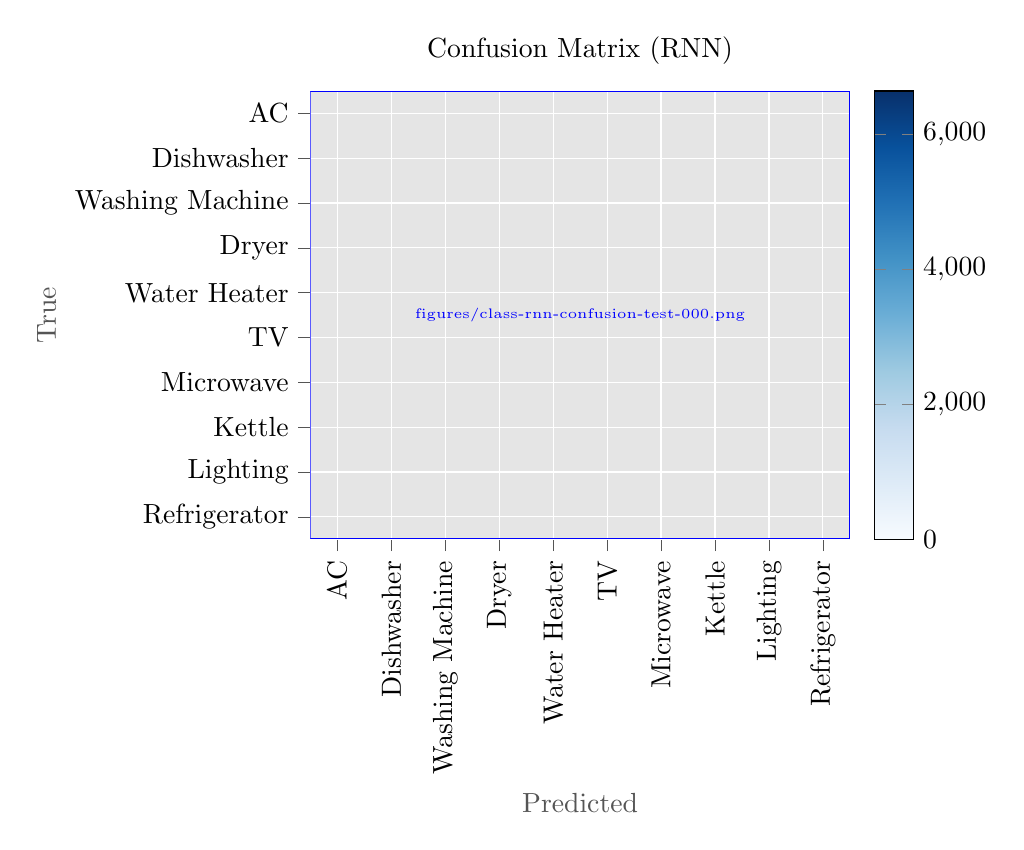
\begin{tikzpicture}

\definecolor{dimgray85}{RGB}{85,85,85}
\definecolor{gainsboro229}{RGB}{229,229,229}

\begin{axis}[
axis background/.style={fill=gainsboro229},
axis line style={white},
colorbar,
colorbar style={ylabel={}},
colormap={mymap}{[1pt]
  rgb(0pt)=(0.968627450980392,0.984313725490196,1);
  rgb(1pt)=(0.870588235294118,0.92156862745098,0.968627450980392);
  rgb(2pt)=(0.776470588235294,0.858823529411765,0.937254901960784);
  rgb(3pt)=(0.619607843137255,0.792156862745098,0.882352941176471);
  rgb(4pt)=(0.419607843137255,0.682352941176471,0.83921568627451);
  rgb(5pt)=(0.258823529411765,0.572549019607843,0.776470588235294);
  rgb(6pt)=(0.129411764705882,0.443137254901961,0.709803921568627);
  rgb(7pt)=(0.0313725490196078,0.317647058823529,0.611764705882353);
  rgb(8pt)=(0.0313725490196078,0.188235294117647,0.419607843137255)
},
point meta max=6638,
point meta min=0,
tick align=outside,
tick pos=left,
title={Confusion Matrix (RNN)},
x grid style={white},
xlabel=\textcolor{dimgray85}{Predicted},
xmajorgrids,
xmin=0, xmax=10,
xtick style={color=dimgray85},
xtick={0.5,1.5,2.5,3.5,4.5,5.5,6.5,7.5,8.5,9.5},
xticklabel style={rotate=90.0},
xticklabels={
  AC,
  Dishwasher,
  Washing Machine,
  Dryer,
  Water Heater,
  TV,
  Microwave,
  Kettle,
  Lighting,
  Refrigerator
},
y dir=reverse,
y grid style={white},
ylabel=\textcolor{dimgray85}{True},
ymajorgrids,
ymin=0, ymax=10,
ytick style={color=dimgray85},
ytick={0.5,1.5,2.5,3.5,4.5,5.5,6.5,7.5,8.5,9.5},
yticklabels={
  AC,
  Dishwasher,
  Washing Machine,
  Dryer,
  Water Heater,
  TV,
  Microwave,
  Kettle,
  Lighting,
  Refrigerator
}
]
\addplot graphics [includegraphics cmd=\pgfimage,xmin=0, xmax=10, ymin=10, ymax=0] {figures/class-rnn-confusion-test-000.png};
\end{axis}

\end{tikzpicture}

  \captionConfusion{ Matrix for the test data}
\end{figure}


%The accuracy in Question 2.1 manifests how the model works for all the appliance as a whole.You also need to show how the classification works for each appliance. To do so, you need to generate the confusion matrix of the classification result, both for the model training and testing. The confusion matrix should present the classification accuracy for each appliance.

\section{Classification using LSTM}

%Keep the same settings as in Question 2.1 and 2.2, except that you use LSTM when implementing federated learning. You then show the simulation plots as required in Question 2.1 and 2.2, and compare with the results when using RNN.

\begin{figure}[H]
  \centering
    \input{report/figures/class-lstm-accuracy}
  \caption{Plot showing the change in accuracy during training}
\end{figure}

\begin{figure}[H]
  \centering
    % This file was created with tikzplotlib v0.10.1.
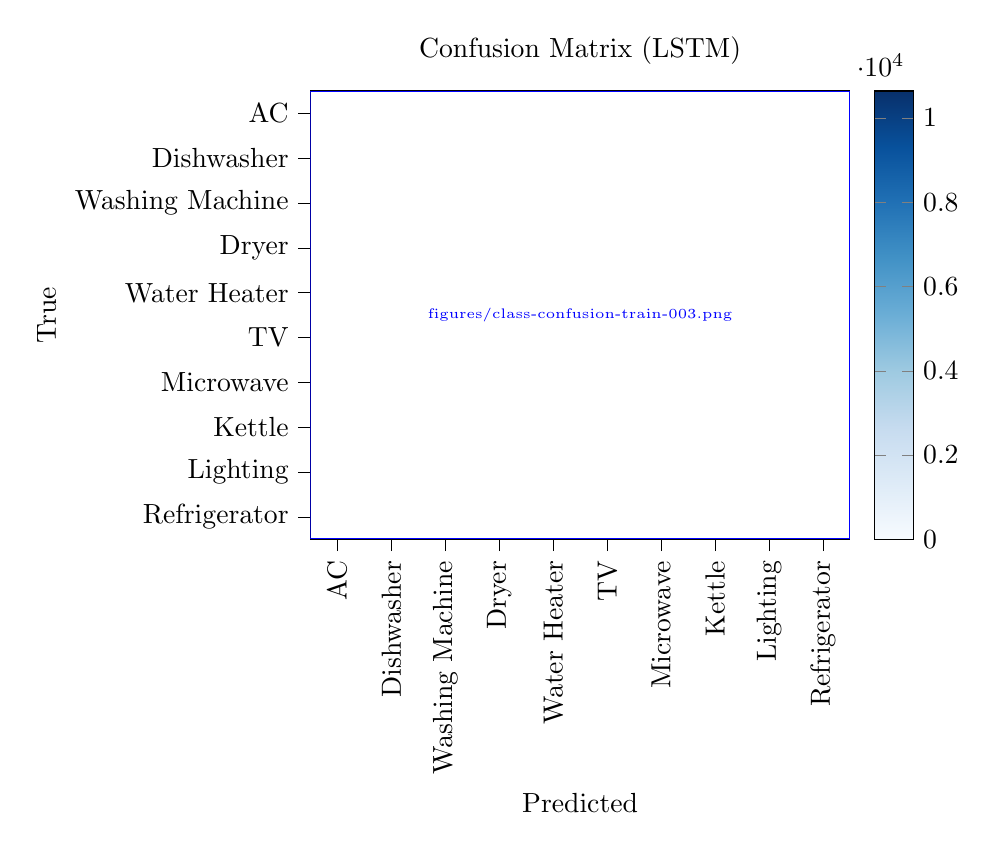
\begin{tikzpicture}

\definecolor{darkgray176}{RGB}{176,176,176}

\begin{axis}[
colorbar,
colorbar style={ylabel={}},
colormap={mymap}{[1pt]
  rgb(0pt)=(0.968627450980392,0.984313725490196,1);
  rgb(1pt)=(0.870588235294118,0.92156862745098,0.968627450980392);
  rgb(2pt)=(0.776470588235294,0.858823529411765,0.937254901960784);
  rgb(3pt)=(0.619607843137255,0.792156862745098,0.882352941176471);
  rgb(4pt)=(0.419607843137255,0.682352941176471,0.83921568627451);
  rgb(5pt)=(0.258823529411765,0.572549019607843,0.776470588235294);
  rgb(6pt)=(0.129411764705882,0.443137254901961,0.709803921568627);
  rgb(7pt)=(0.0313725490196078,0.317647058823529,0.611764705882353);
  rgb(8pt)=(0.0313725490196078,0.188235294117647,0.419607843137255)
},
point meta max=10644,
point meta min=0,
tick align=outside,
tick pos=left,
title={Confusion Matrix (LSTM)},
x grid style={darkgray176},
xlabel={Predicted},
xmin=0, xmax=10,
xtick style={color=black},
xtick={0.5,1.5,2.5,3.5,4.5,5.5,6.5,7.5,8.5,9.5},
xticklabel style={rotate=90.0},
xticklabels={
  AC,
  Dishwasher,
  Washing Machine,
  Dryer,
  Water Heater,
  TV,
  Microwave,
  Kettle,
  Lighting,
  Refrigerator
},
y dir=reverse,
y grid style={darkgray176},
ylabel={True},
ymin=0, ymax=10,
ytick style={color=black},
ytick={0.5,1.5,2.5,3.5,4.5,5.5,6.5,7.5,8.5,9.5},
yticklabels={
  AC,
  Dishwasher,
  Washing Machine,
  Dryer,
  Water Heater,
  TV,
  Microwave,
  Kettle,
  Lighting,
  Refrigerator
}
]
\addplot graphics [includegraphics cmd=\pgfimage,xmin=0, xmax=10, ymin=10, ymax=0] {figures/class-confusion-train-003.png};
\end{axis}

\end{tikzpicture}

  \captionConfusion {Matrix for the training data}
\end{figure}

\begin{figure}[H]
  \centering
    \input{report/figures/class-lstm-confusion-test}
  \captionConfusion {Matrix for the test data}
\end{figure}



\chapter{Conclusion}

In both the prediction model and classification model, we can see that LSTM outperforms RNN. LSTM, however, has a more complex architecture, and takes more epochs and execution time. For the prediction model, this added complexity is well worth the added execution time as the results are considerable better at picking up the patterns as evident when comparing them to the ground truth. For the classification model, this distinction isn't as clear cut. We can see that the LSTM model still outperforms RNN in accuracy, but this marginal gain is not as significant. This might be due to how the classification model only considers a day, instead of having a whole week for its time series. LSTM's ability to retain long term dependencies in the data is therefore not as advantageous as in the prediction model.

\nocite{tensorflow2015-whitepaper}
\nocite{dataset}

\printbibliography{}

\vspace*{10mm}
\end{document}